% A. Tipo de documento
	\documentclass[12pt]{article} %estilo de documento
	
% C. Formato de párrafos
	\usepackage[top=3cm, bottom=2.5cm, left=2.5cm, right=2.5cm]{geometry}  % márgenes
	
\usepackage{graphicx} %gráficos
\usepackage{float}      %ubicación

\usepackage[T1]{fontenc}
\usepackage[spanish]{babel}
\usepackage[utf8]{inputenc}


\usepackage{mathpazo,amsmath,mathtools,graphicx,xcolor,array,pdfpages,float}
\usepackage{xcolor,setspace, subcaption,titlesec,longtable,titletoc, comment}
\usepackage{array,multirow,graphicx,enumitem}
\usepackage{hyperref}
\pagestyle{myheadings}

% Bibliography
%\usepackage[english]{babel}

% Hipervinculos
\definecolor{udesa}{HTML}{00529B}
\usepackage[colorlinks=true, allcolors=udesa]{hyperref}
%\usepackage{listings}
\usepackage[colorinlistoftodos]{todonotes}
\usepackage{parskip}
\definecolor{coolblack}{rgb}{0.0, 0.18, 0.39}
\definecolor{darkcerulean}{rgb}{0.03, 0.27, 0.49}
\definecolor{frenchblue}{rgb}{0.0, 0.45, 0.73}
\definecolor{indigo(dye)}{rgb}{0.0, 0.25, 0.42}
\definecolor{officegreen}{rgb}{0.0, 0.5, 0.0}
\markboth{4444}{Herramientas computacionales para la investigaci\'on - UdeSA}

\begin{document}



\begin{titlepage} % Suppresses displaying the page number on the title page and the subsequent page counts as page 1
	\newcommand{\HRule}{\rule{\linewidth}{0.5mm}} % Defines a new command for horizontal lines, change thickness here
	
	\center % Centre everything on the page
	
	%------------------------------------------------
	%	Headings
	%------------------------------------------------
	
\includegraphics[width=0.7\textwidth]{UdeSA.jpg}
	
	\textsc{\Large Herramientas computacionales de investigaci\'on  }\\[0.5cm] % Major heading such as course name
	
	\textsc{\large Profesora:María Amelia Gibbons }\\
	\vspace{0,15cm}
	\vspace{4pt}
	
	%------------------------------------------------
	%	Title
	%------------------------------------------------
	\textcolor{white}{\HRule}\\[0.6cm]
	\huge\bfseries Trabajo Práctico N$^{o}$2
	\textcolor{white}{\HRule}\\[1.5cm]
	%------------------------------------------------
	%	Author(s)
	%------------------------------------------------
	\begin{center}
		\large
		\textsc{Luis Cerda y Gonzalo Rigirozzi}\\
	\end{center}
	
	%------------------------------------------------
	%	Date
	%------------------------------------------------
	\vfill\vfill\vfill % Position the date 3/4 down the remaining page
	{\large 10 de Julio de 2022}
	\vfill
	
\end{titlepage}

\section {Datos georeferenciados de la ciudad de Chicago}

A partir de los datos brindados en clase, se procedió a elaborar 3 mapas y 3 gráficos con la información georreferenciada de la Ciudad de Chicago. Mediante esta técnica, es posible generar información para el análisis espacial y de esta forma encontrar patrones que sirvan para la toma de decisiones y elaboración de políticas.

\subsection{Mapas de la Ciudad de Chicago}

En el siguiente mapa se muestra cantidad de hogares bajo la linea de pobreza en cada \textit{community} de la Ciudad de Chicago. La escala cromatica, nos indicada que a mayor intensidad, aumenta el numero de hogares bajo la linea de pobreza.
     

\begin{figure}[H]
	\centering
	\begin{minipage}{0.64\textwidth}
		\centering
		%\captionsetup{labelformat=empty}
		\caption{\textbf{Porcentaje de hogares bajo la linea de pobreza}}
		%\label{fig:Grafico 1}
		\includegraphics[,width=1\linewidth]{./pobreza} %Poner el nombre del gráfico sin su extensión
		\begin{flushleft}
			{\footnotesize Fuente: Chicago Data Portal.}
		\end{flushleft}
\end{minipage} \end{figure} 
    
Asi mismo, en el siguiente mapa muestra el precio por persona en USD de alquiler para Airbnb en la Ciudad de Chicago. Se puede apreciar, que en su mayoria las \textit{community} costeras, y que a su vez tienen menos hogares bajo la linea de pobreza, tienen precios más altos para hospedarse. Nuevamente se utiliza una escala cromatica, y se divide en 5 categorias dependiendo el precio por persona. Al igual que en el caso anterior, a colores más oscuros se corresponde con precios mas altos de hospedaje por persona.

\begin{figure}[H]
	\centering
	\begin{minipage}{0.65\textwidth}
		\centering
		%\captionsetup{labelformat=empty}
		\caption{\textbf{Precio de Airbnb por persona en USD}}
		%\label{fig:Grafico 1}
		\includegraphics[,width=1\linewidth]{./price} %Poner el nombre del gráfico sin su extensión
		\begin{flushleft}
			{\footnotesize Fuente: Chicago Data Portal.}
		\end{flushleft}
\end{minipage} \end{figure} 

Continuando con este analisis, en el siguiente mapa se muestra el número total de robos. Similar a los anteriores se ve en las zonas con mas robos mayor intensidad crom\'atica. Se categoriz\'o en 5 niveles. La idea de agregar el este mapa y contrastarlo con los anteriores, surge que a partir de ellos se puede hacer un an\'alisis detallado de las \textit{community} de Chicago. Se puede ver que las \textit{community} con menos hogares bajo la linea de pobreza (figura 1), y que a su vez tienen precios en USD mas bajos, son en general \textit{community} que reflejan menos números de robo, un ejemplo de ello es \textit{Roseland}. A su vez las \textit{community} con mayor precio de hospedaje en USD por persona, y que a su vez tienen menos hogares bajo la lina de pobreza, muestran mayor cantidad de robos, como por ejemplo \textit{Lakeview, Lincoln Park y Near North Side}.


\begin{figure}[H]
	\centering
	\begin{minipage}{0.65\textwidth}
		\centering
		%\captionsetup{labelformat=empty}
		\caption{\textbf{Precio de Airbnb por persona en USD}}
		%\label{fig:Grafico 1}
		\includegraphics[,width=1\linewidth]{./theft} %Poner el nombre del gráfico sin su extensión
		\begin{flushleft}
			{\footnotesize Fuente: Chicago Data Portal.}
		\end{flushleft}
\end{minipage} \end{figure}



\subsection{Gráficos para la Ciudad de Chicago}

En el siguiente gráfico se muestra la tasa de aceptaci\'on de los host de Airbnb.

\begin{figure}[H]
	\centering
	\begin{minipage}{0.65\textwidth}
		\centering
		%\captionsetup{labelformat=empty}
		\caption{\textbf{Tasa de aceptación de reservas en Airbnb}}
		%\label{fig:Grafico 1}
		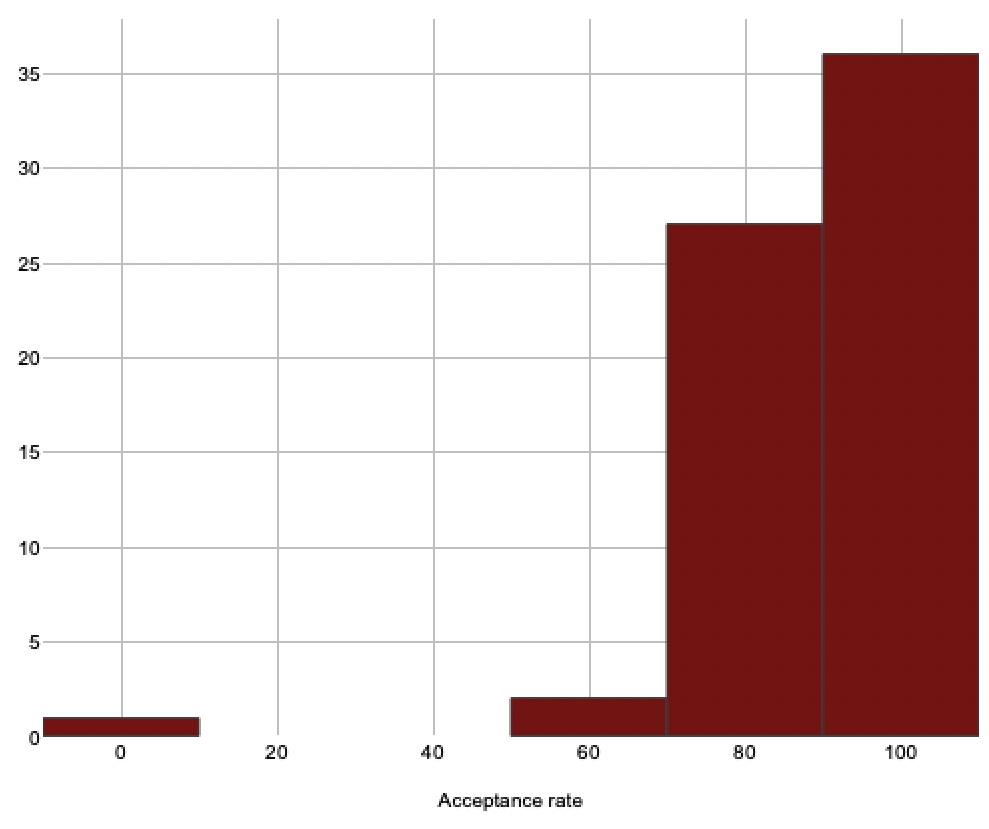
\includegraphics[,width=1\linewidth]{./GRAFacceptance_rate} %Poner el nombre del gráfico sin su extensión
		\begin{flushleft}
			{\footnotesize Fuente: Chicago Data Portal.}
		\end{flushleft}
\end{minipage} \end{figure}


Así mismo, en el siguiente gráfico se muestra el número de hogares bajo la linea de pobreza dentro de cada \textit{community}. En contexto con los mapas de la seccion anterior, se ve que las \textit{community} costeras presentan menos hogares bajo la linea de pobreza.

\begin{figure}[H]
	\centering
	\begin{minipage}{0.65\textwidth}
		\centering
		%\captionsetup{labelformat=empty}
		\caption{\textbf{Hogares bajo la l\'inea de pobreza por comunidad}}
		%\label{fig:Grafico 1}
		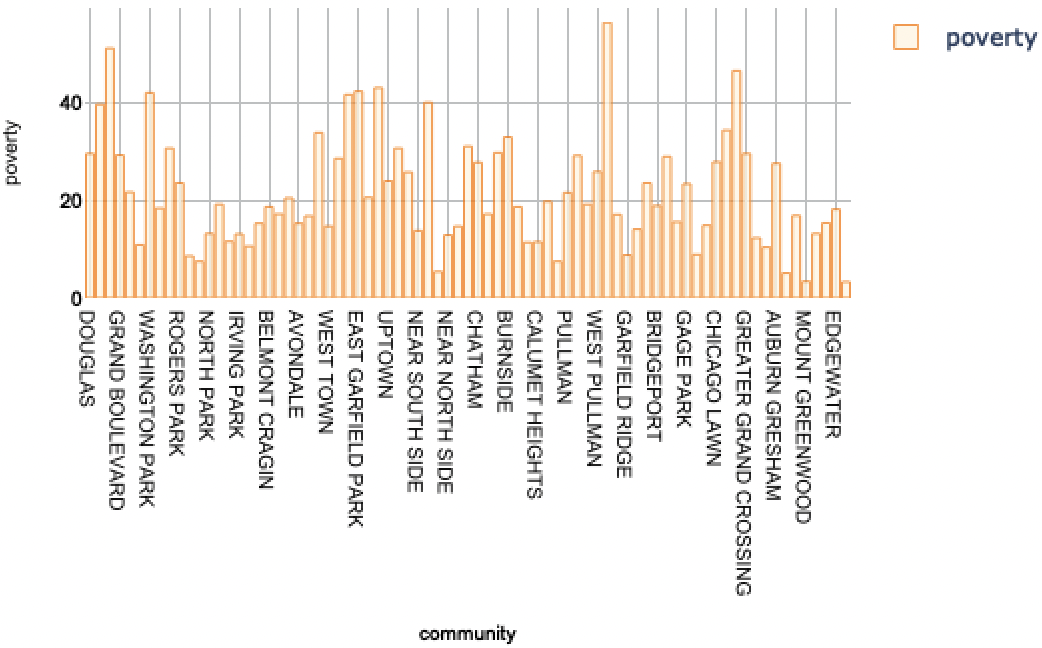
\includegraphics[,width=1\linewidth]{./GRAFcommunity} %Poner el nombre del gráfico sin su extensión
		\begin{flushleft}
			{\footnotesize Fuente: Chicago Data Portal.}
		\end{flushleft}
\end{minipage} \end{figure}


Finalmente, se intenta mostrar la relaci\'on entre hogares bajo la linea de pobreza, y cantidad de total de robos. Se aprecia cierta relaci\'on posit\'iva entre las variables, pero como se decribi\'o anteriormente en la secci\'on de mapas, los \textit{community} con mayor cantidad total de robos no eran necesariamente los de mayor pobreza, y este grafico, da sustento a esta hip\'otesis.
    
\begin{figure}[H]
	\centering
	\begin{minipage}{0.65\textwidth}
		\centering
		%\captionsetup{labelformat=empty}
		\caption{\textbf{Relaci\'on pobreza y número total de robos}}
		%\label{fig:Grafico 1}
		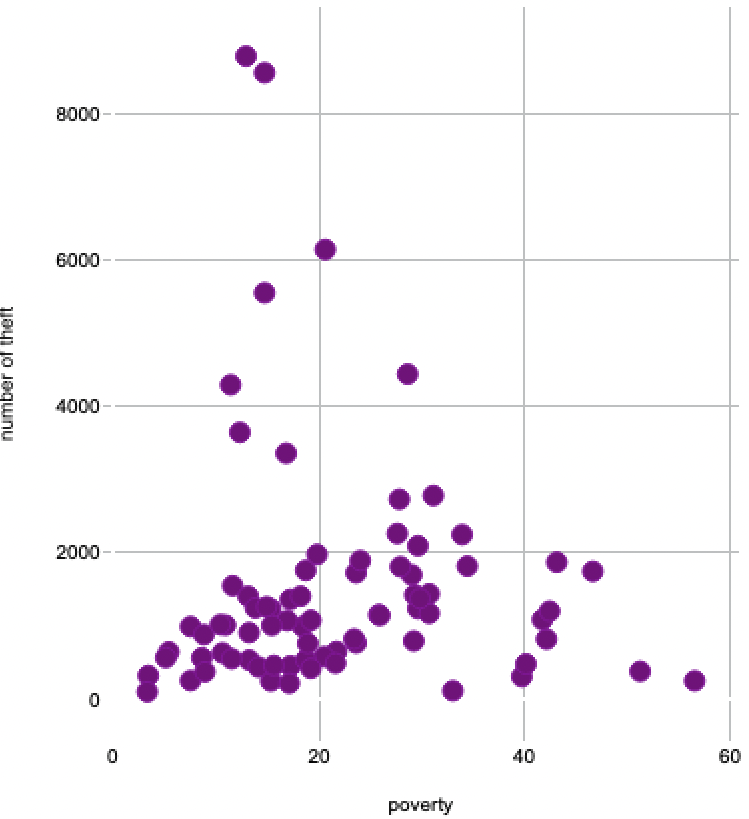
\includegraphics[,width=1\linewidth]{./GRAFtheft_poverty} %Poner el nombre del gráfico sin su extensión
		\begin{flushleft}
			{\footnotesize Fuente: Chicago Data Portal.}
		\end{flushleft}
\end{minipage} \end{figure}

\newpage

\section{{Aplicaci\'on para la Provincia de Buenos Aires}}

A partir de la información del Censo Nacional de Población, Hogares y Viviendas 2010 disponible en la página web del Instituto Nacional de Estadísticas y Censos (INDEC), se elaboraron dos mapas de calor para los partidos que conforman la Provincia de Buenos Aires. Específicamente, para la representación de estos mapas se utilizaron las variables de desocupados y de hogares con necesidades básicas insatisfechas (NBI), ambas como porcentaje del total por partido.\\

Este ejercicio resulta pertinente por la cantidad de personas que aglutina la Provincia de Buenos Aires, siendo esta la más habitada de la República Argentina. De esta forma, con base en la información del Censo de 2010, la Provincia de Buenos Aires contaba con 15,625,084 habitantes, lo que representa el 38.9 por ciento de la población total Argentina. De estos 15,625,084 de habitantes, 11,928,986 viven en lo que se denomina la Región Metropolitana de Buenos Aires (RMBA). Así, la población de la RMBA representa el 76.3 por ciento del total de la Provincia y el 29.7 por ciento de la población total Argentina.\footnote{Argentina, I. N. D. E. C. ``Censo Nacional de Población, Hogares y Viviendas 2010''. Recuperado de https://www.indec.gob.ar/ftp/cuadros/poblacion/censo2010\_tomo1.pdf}\\

En línea con lo anterior, se presenta la figura 7 en donde se muestra el mapa por quintiles del porcentaje de desocupados a nivel de partidos. Lo destacable de este mapa, es que se evidencia como la aglomeración poblacional registrada en la RMBA tiene un efecto sobre la tasa de desocupación de sus habitantes, registrando los partidos con más desempleo en toda la provincia.\\

\begin{figure}[H]
	\centering
	\begin{minipage}{0.6\textwidth}
		\centering
		%\captionsetup{labelformat=empty}
		\caption{\textbf{Desocupados por partido}}
		%\label{fig:Grafico 1}
		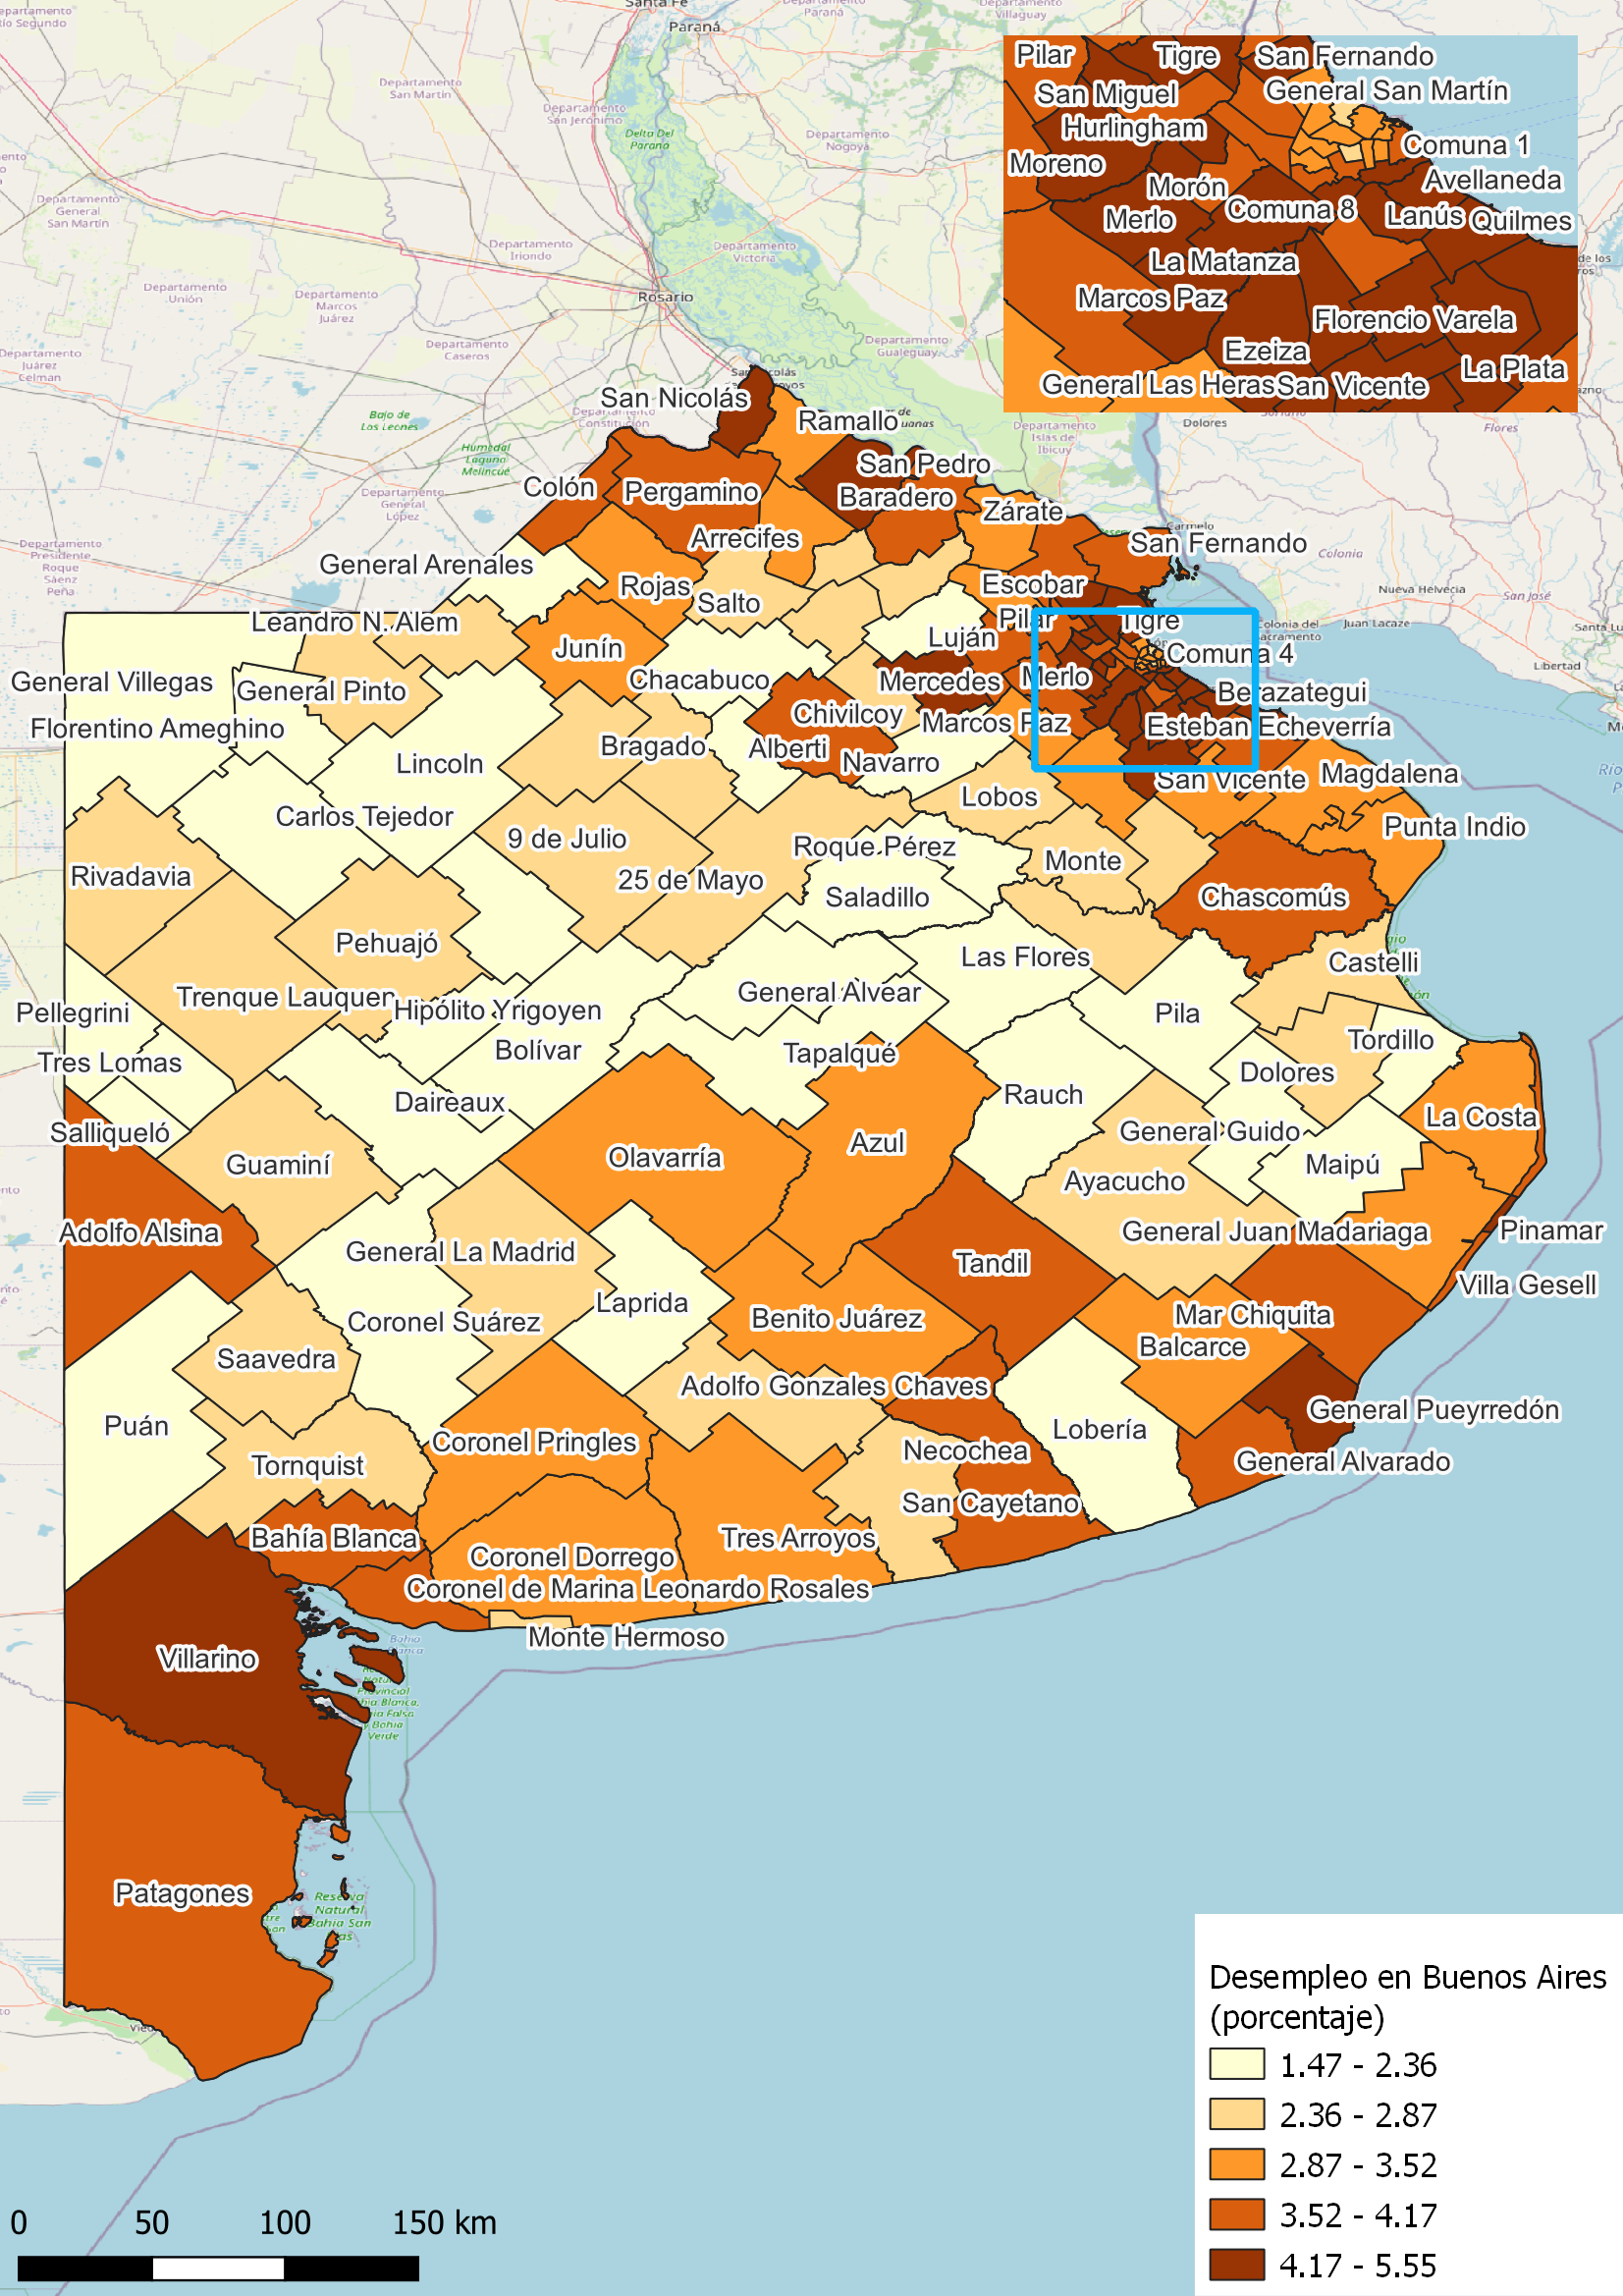
\includegraphics[,width=1\linewidth]{./desempleo2_bsas} %Poner el nombre del gráfico sin su extensión
		\begin{flushleft}
			{\footnotesize Fuente: INDEC.}
		\end{flushleft}
\end{minipage} \end{figure}


Así mismo, se presenta la figura 8 en donde se muestra, utilizando la misma agrupación por quintiles como en el mapa anterior, el indicador de hogares con necesidades básicas insatisfechas, este indicador permite aproximar la pobreza no solo teniendo en cuenta los ingresos, sino además falta absoluta de acceso a cuestiones consideradas básicas\footnote{Argentina, I. N. D. E. C. ``Censo Nacional de Población, Hogares y Viviendas 2010''. Recuperado de https://www.indec.gob.ar/ftp/cuadros/poblacion/censo2010\_tomo1.pdf}. Los resultados de este mapa no difieren mucho del anterior respecto a que RMBA, siendo estos los partidos con mayores porcentajes de ausencia absoluta de NBI. Aquí cabe resaltar que dentro de esta sub región, los partidos de Comuna 2, 6, 11, 12, 13, 14 y Vicente López son quienes presenta menor porcentaje de NBI.\\

\begin{figure}[H]
	\centering
	\begin{minipage}{0.6\textwidth}
		\centering
		%\captionsetup{labelformat=empty}
		\caption{\textbf{Necesidades básicas insatisfechas por partido}}
		%\label{fig:Grafico 1}
		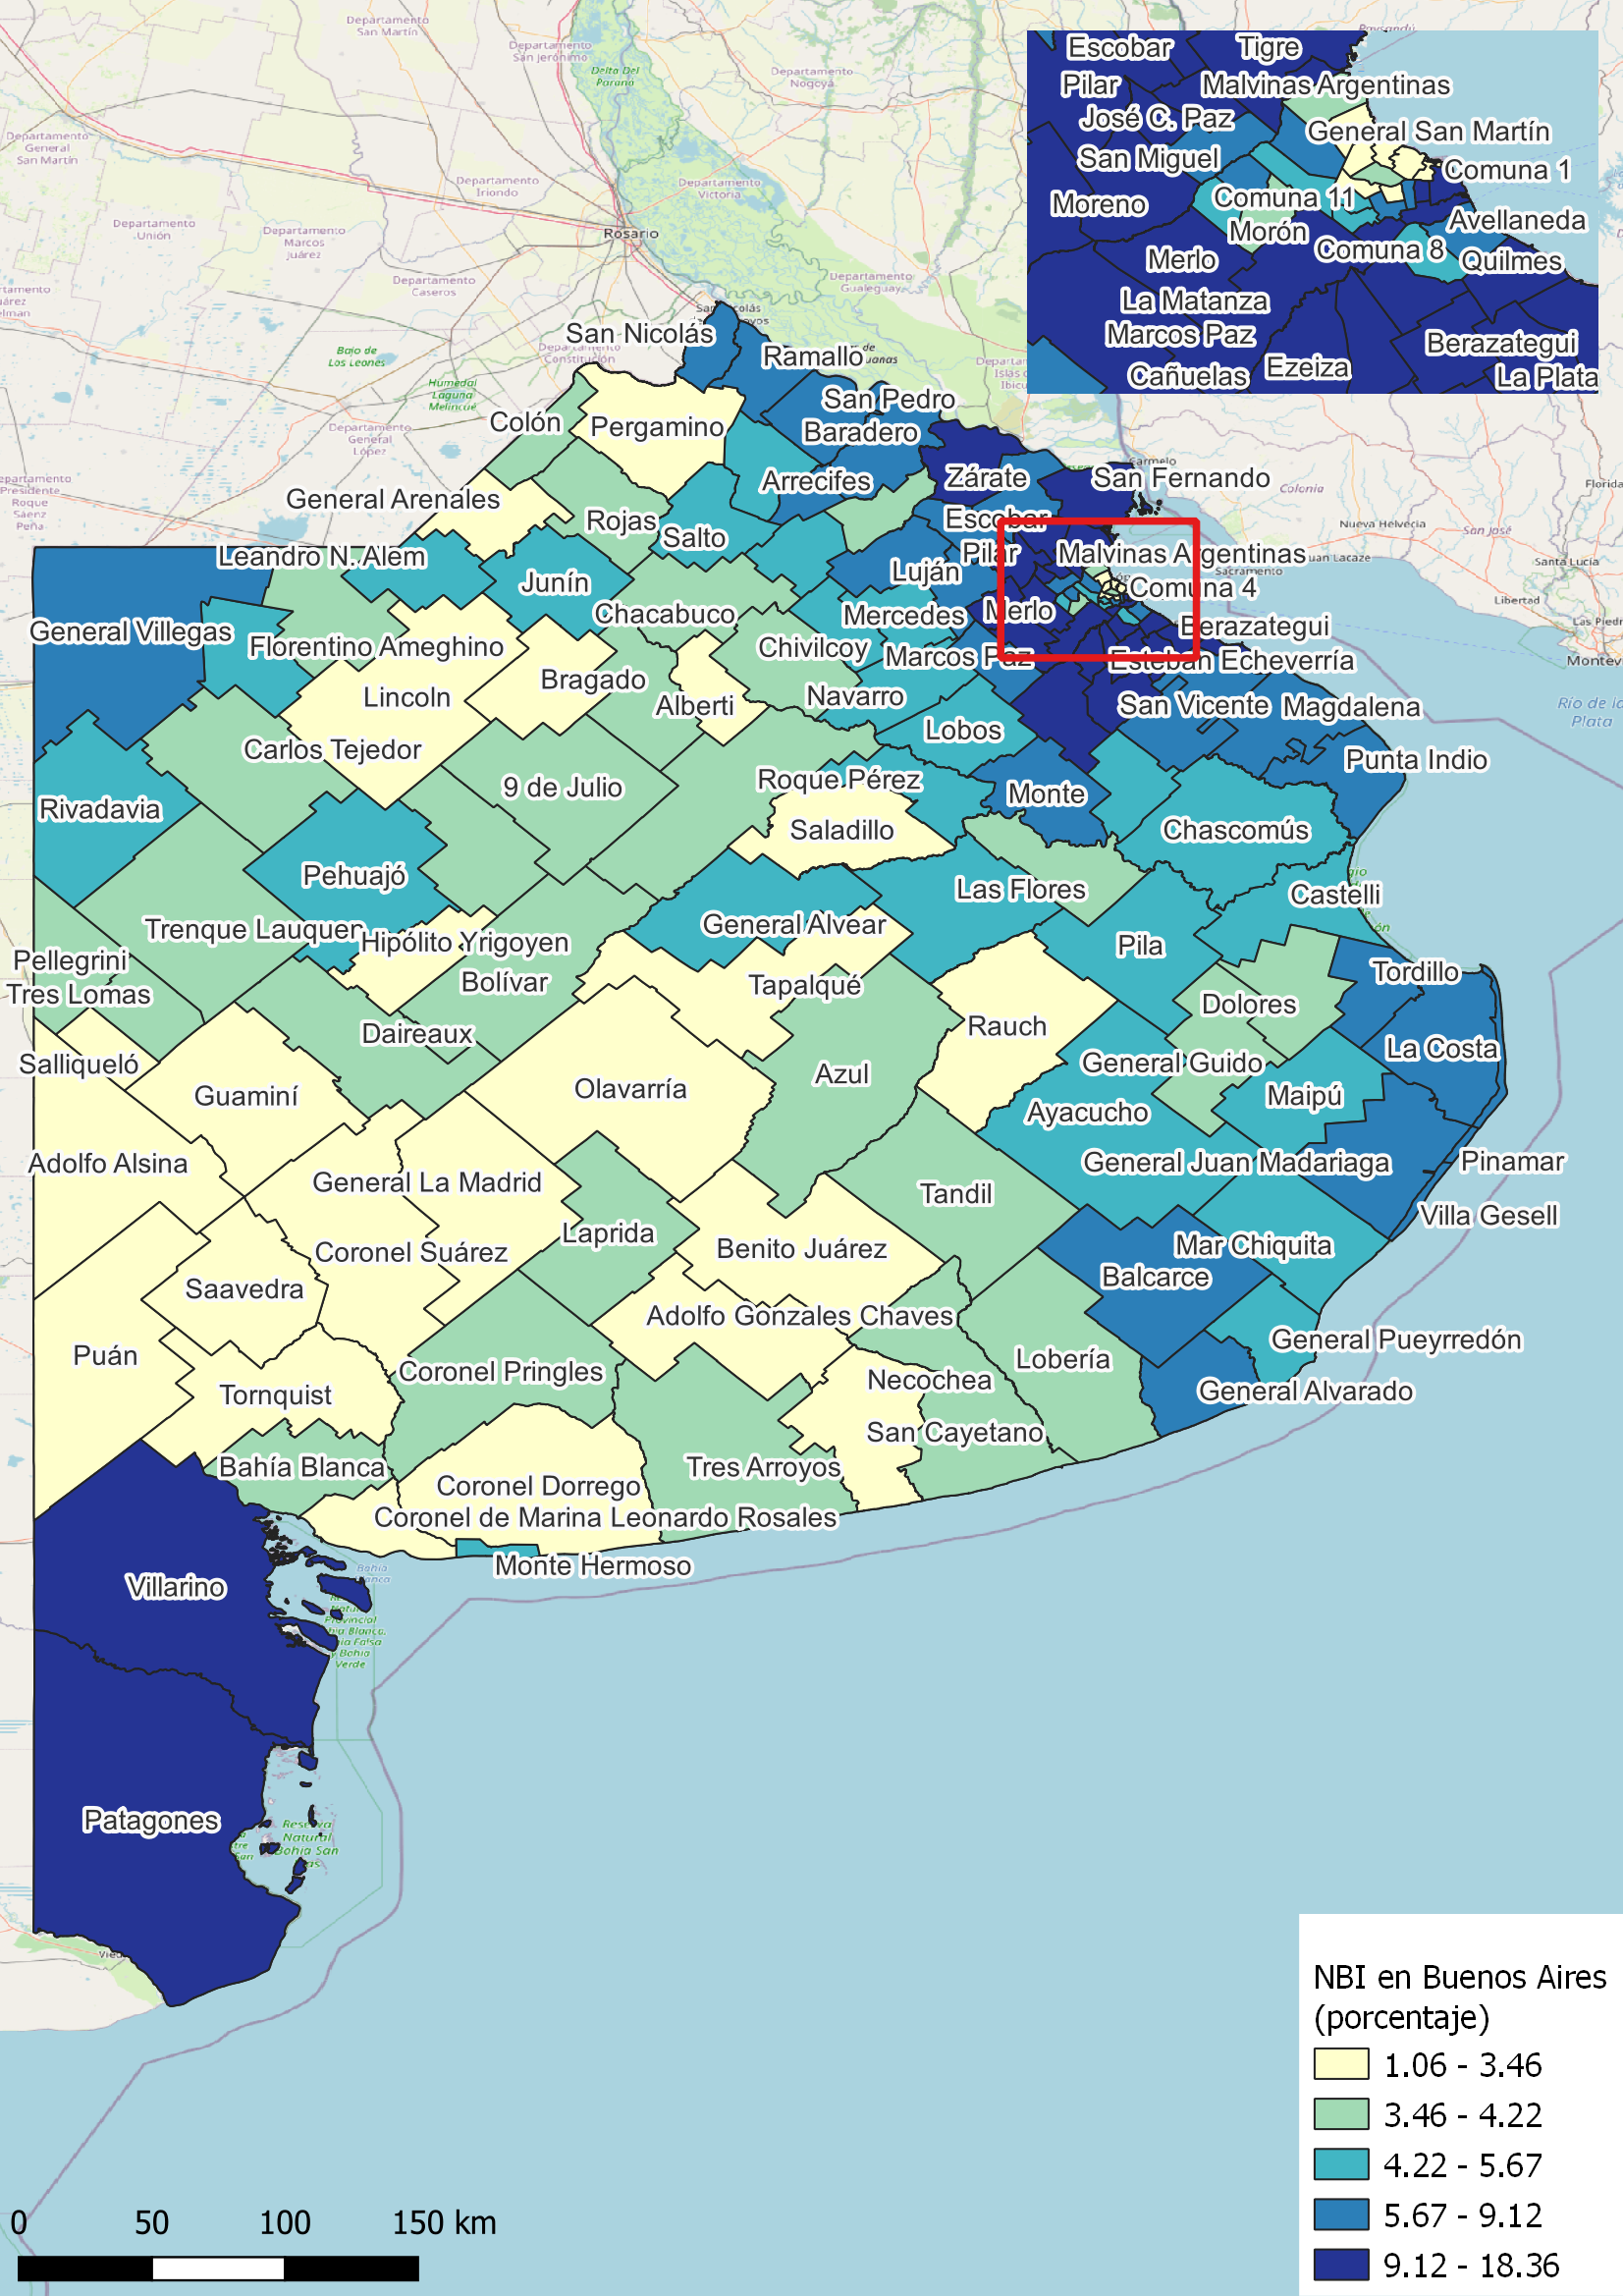
\includegraphics[,width=1\linewidth]{./nbi_bsas_v2} %Poner el nombre del gráfico sin su extensión
		\begin{flushleft}
			{\footnotesize Fuente: INDEC.}
		\end{flushleft}
\end{minipage} \end{figure}

Finalmente, este pequeño ejercicio pudiera servir de referencia para compararse con los resultados del reciente Censo realizado en mayo de 2022. La actualización de estos datos podrá reflejar la evolución temporal de estas variables en 12 años y servir como punto de partida para el análisis, evaluación y elaboración de políticas públicas. 


\end{document}



















